\documentclass[11pt]{article} 
\def\names{Hunter Kruger-Ilingworth (14198489)\\ 
Quentin Bouet (14198423) \\
Thomas Mehes (14259613) \\}
\def\doctitle{Assignment 2 \\ Dew Point Generator Controller and Sensor Data Logger}
\def\subjectcode{CC3501}
% Geometry and Layout
    \usepackage[margin=0.75in]{geometry}
    \usepackage{multicol}

% Graphics and Diagrams
    \usepackage{xcolor}
    \usepackage{graphicx} % Required for inserting images
    \usepackage[american]{circuitikz}
    \usepackage{tikz}
    \usepackage{tikz-3dplot}
    \usetikzlibrary{arrows.meta}
    \usepackage{pgfplots}
    \pgfplotsset{compat=newest}
    \usepackage{listings}
    \usepackage{tcolorbox}

% CSV Table input
    \usepackage{csvsimple, booktabs}

% Code Chunk Formatting
    \definecolor{comment_color}{rgb}{0.52,0.38,0.78}
    \definecolor{keyword_color}{rgb}{0.84,0.27,0.3}
    \definecolor{background_color}{rgb}{0.95,0.95,0.95}
    \usepackage{inconsolata} % Consolas-style font from the inconsolata package

\lstset{
    backgroundcolor=\color{background_color},   % Choose the background color
    commentstyle=\color{comment_color},       % Style of comments
    keywordstyle=\color{keyword_color},        % Style of keywords
    stringstyle=\color{red},              % Style of strings, assuming red
    basicstyle=\footnotesize\ttfamily, % Set font size, monospaced font, and color        
    breakatwhitespace=false,              % Automatic line breaking only at whitespace
    breaklines=true,                      % Automatic line breaking
    captionpos=t,                         % Caption position is on top
    keepspaces=true,                      % Keeps spaces in text
    numbers=left,                         % Line number position
    numbersep=5pt,                        % How far the line numbers are from the code
    showspaces=false,                     % Show spaces in the code
    showstringspaces=false,               % Underline spaces within strings only
    showtabs=false,                       % Show tabs within strings adding particular underscores
    tabsize=2,                            % Sets default tab size
    title=\lstname                        % Show the filename of files included with \lstinputlisting
}
% Text Content / Math
    \usepackage{lipsum} % Dummy text
    \usepackage{hyperref}
    \usepackage{amsmath} % For sum symbol and other math formatting

% Headers and Footers
    \usepackage{lastpage}
    \usepackage{fancyhdr}
    \makeatletter
    \renewcommand{\@seccntformat}[1]{}
    \makeatother
    \pagestyle{fancy}
    \fancyhf{} 
    \setlength{\headheight}{15pt}
    \fancyhead[L]{\subjectcode{} - \doctitle{}}
    \fancyhead[R]{} % Rearrange as you please
    \fancyfoot[L]{\name{}}
    \fancyfoot[R]{Page \thepage\ of \pageref{LastPage}} 
    \renewcommand{\headrulewidth}{0pt}

% Caption and Referencing Customization
    \usepackage{caption}
    \usepackage{cleveref}
    \DeclareCaptionLabelSeparator{IEEE}{.\quad }
    \captionsetup[figure]{name=Fig., labelsep=IEEE}
    \captionsetup{format=hang, labelfont=bf}
    \captionsetup{justification=raggedright,singlelinecheck=false}

% Document Metadata and First Page Formatting
    \title{\doctitle{}\\\large{James Cook University Cairns}}
    \author{\name{} (\studentnumber{})\\ 
    Quentin Boet (\note{whatever your number is }) \\
    Thomas Mehes (\note{whatever your number is }) \\}
    \date{\today}

% References
    \usepackage{natbib}


%Choose which files are re-rendered (saves rendering time)
%\includeonly{}

\newcommand{\insertimage}[3]{
\begin{figure}[h]
    \centering
    \includegraphics[width=\linewidth]{#1} % Image filename
    \caption{#2} % Caption
    \label{#3} % Label
\end{figure}
}

\newcommand{\insertbigimage}[3]{
\begin{figure*}[h]
    \centering
    \includegraphics[width=\linewidth]{#1} % Image filename
    \caption{#2} 
    \label{#3} 
\end{figure*}
}

\newcommand{\codeblock}[4]{
    \lstinputlisting[language=#1, caption={#2}, label=#3]{#4}
}


\newcommand{\E}[1]{
    \cdot 10^{#1}
}

\newcommand{\abs}[1]{
    \left\lvert #1 \right\rvert
}

\newcommand{\note}[1]{\textcolor{red}{#1}} %create a note for yourself


\definecolor{codegray}{gray}{0.9} % Light gray color
\newcommand{\code}[1]{\colorbox{codegray}{\texttt{\detokenize{#1}}}} % Command for inline code

\begin{document}
    % Create the title page
    \begin{titlepage}
        \maketitle
        \thispagestyle{empty} %suppresses page numbering on the title page
    \end{titlepage}

    % Table of Contents
    \thispagestyle{empty} % Suppresses page numbering on the contents page
    \onecolumn
    \tableofcontents
    \listoffigures
    \listoftables

    % Document - place new files as needed
    \clearpage
    \section{Intro}

This report details the design and implementation of an embedded system functioning as both a scientific data logger and a smart interface with an analogue dew point generator. Utilizing the RP2040 microcontroller, SDI-12 environmental sensors, and a load cell, the system collects and processes data for climate modelling. The project aims to offer a reliable and efficient solution for monitoring and controlling environmental parameters, especially in researching tropical plant behavior under varying climate conditions.

The LI-610 Dew Point Generator is a precision instrument that produces a stable gas stream with a controlled dew point. It employs Peltier thermoelectric coolers to regulate water reservoir temperatures, ensuring the air stream is fully saturated with water vapor. This precise dew point control is vital in environmental research, preventing condensation in climate-controlled chambers and maintaining experimental conditions and data accuracy.

Accurate, continuous monitoring of environmental parameters is crucial for tropical plant research, but traditional methods are labor-intensive, error-prone, and physical presence in climate-controlled rooms can disrupt experiments. Commercial solutions like Campbell Scientific are often expensive and closed-source, limiting accessibility and customization for researchers. This project provides an open-source, cost-effective alternative for remote monitoring and control. By integrating various sensors and a smart interface for the dew point generator, the system enables the simulation of different climate conditions and monitoring of plant responses without entering the controlled environment, ensuring data integrity while enhancing flexibility and affordability.
    \insertbigimage{figures/block_diagram.pdf}{Block diagram of the system}{block_diagram}

\section{System Design Overview}

The system was designed around the RP2040 microcontroller, acting as the central 
processing unit for interfacing with a variety of sensors and control devices. 
The design incorporates the SF-5M sap flow sensor, LT-1T leaf temperature sensor, 
and MT-603 load cell to measure various environmental parameters. Each of these 
sensors use different communication protocols, requiring careful consideration of 
power requirements, signal integrity, and communication compatibility. \cref{block_diagram} 
shows an overview of all the communication systems involved in the design.

\begin{figure}
    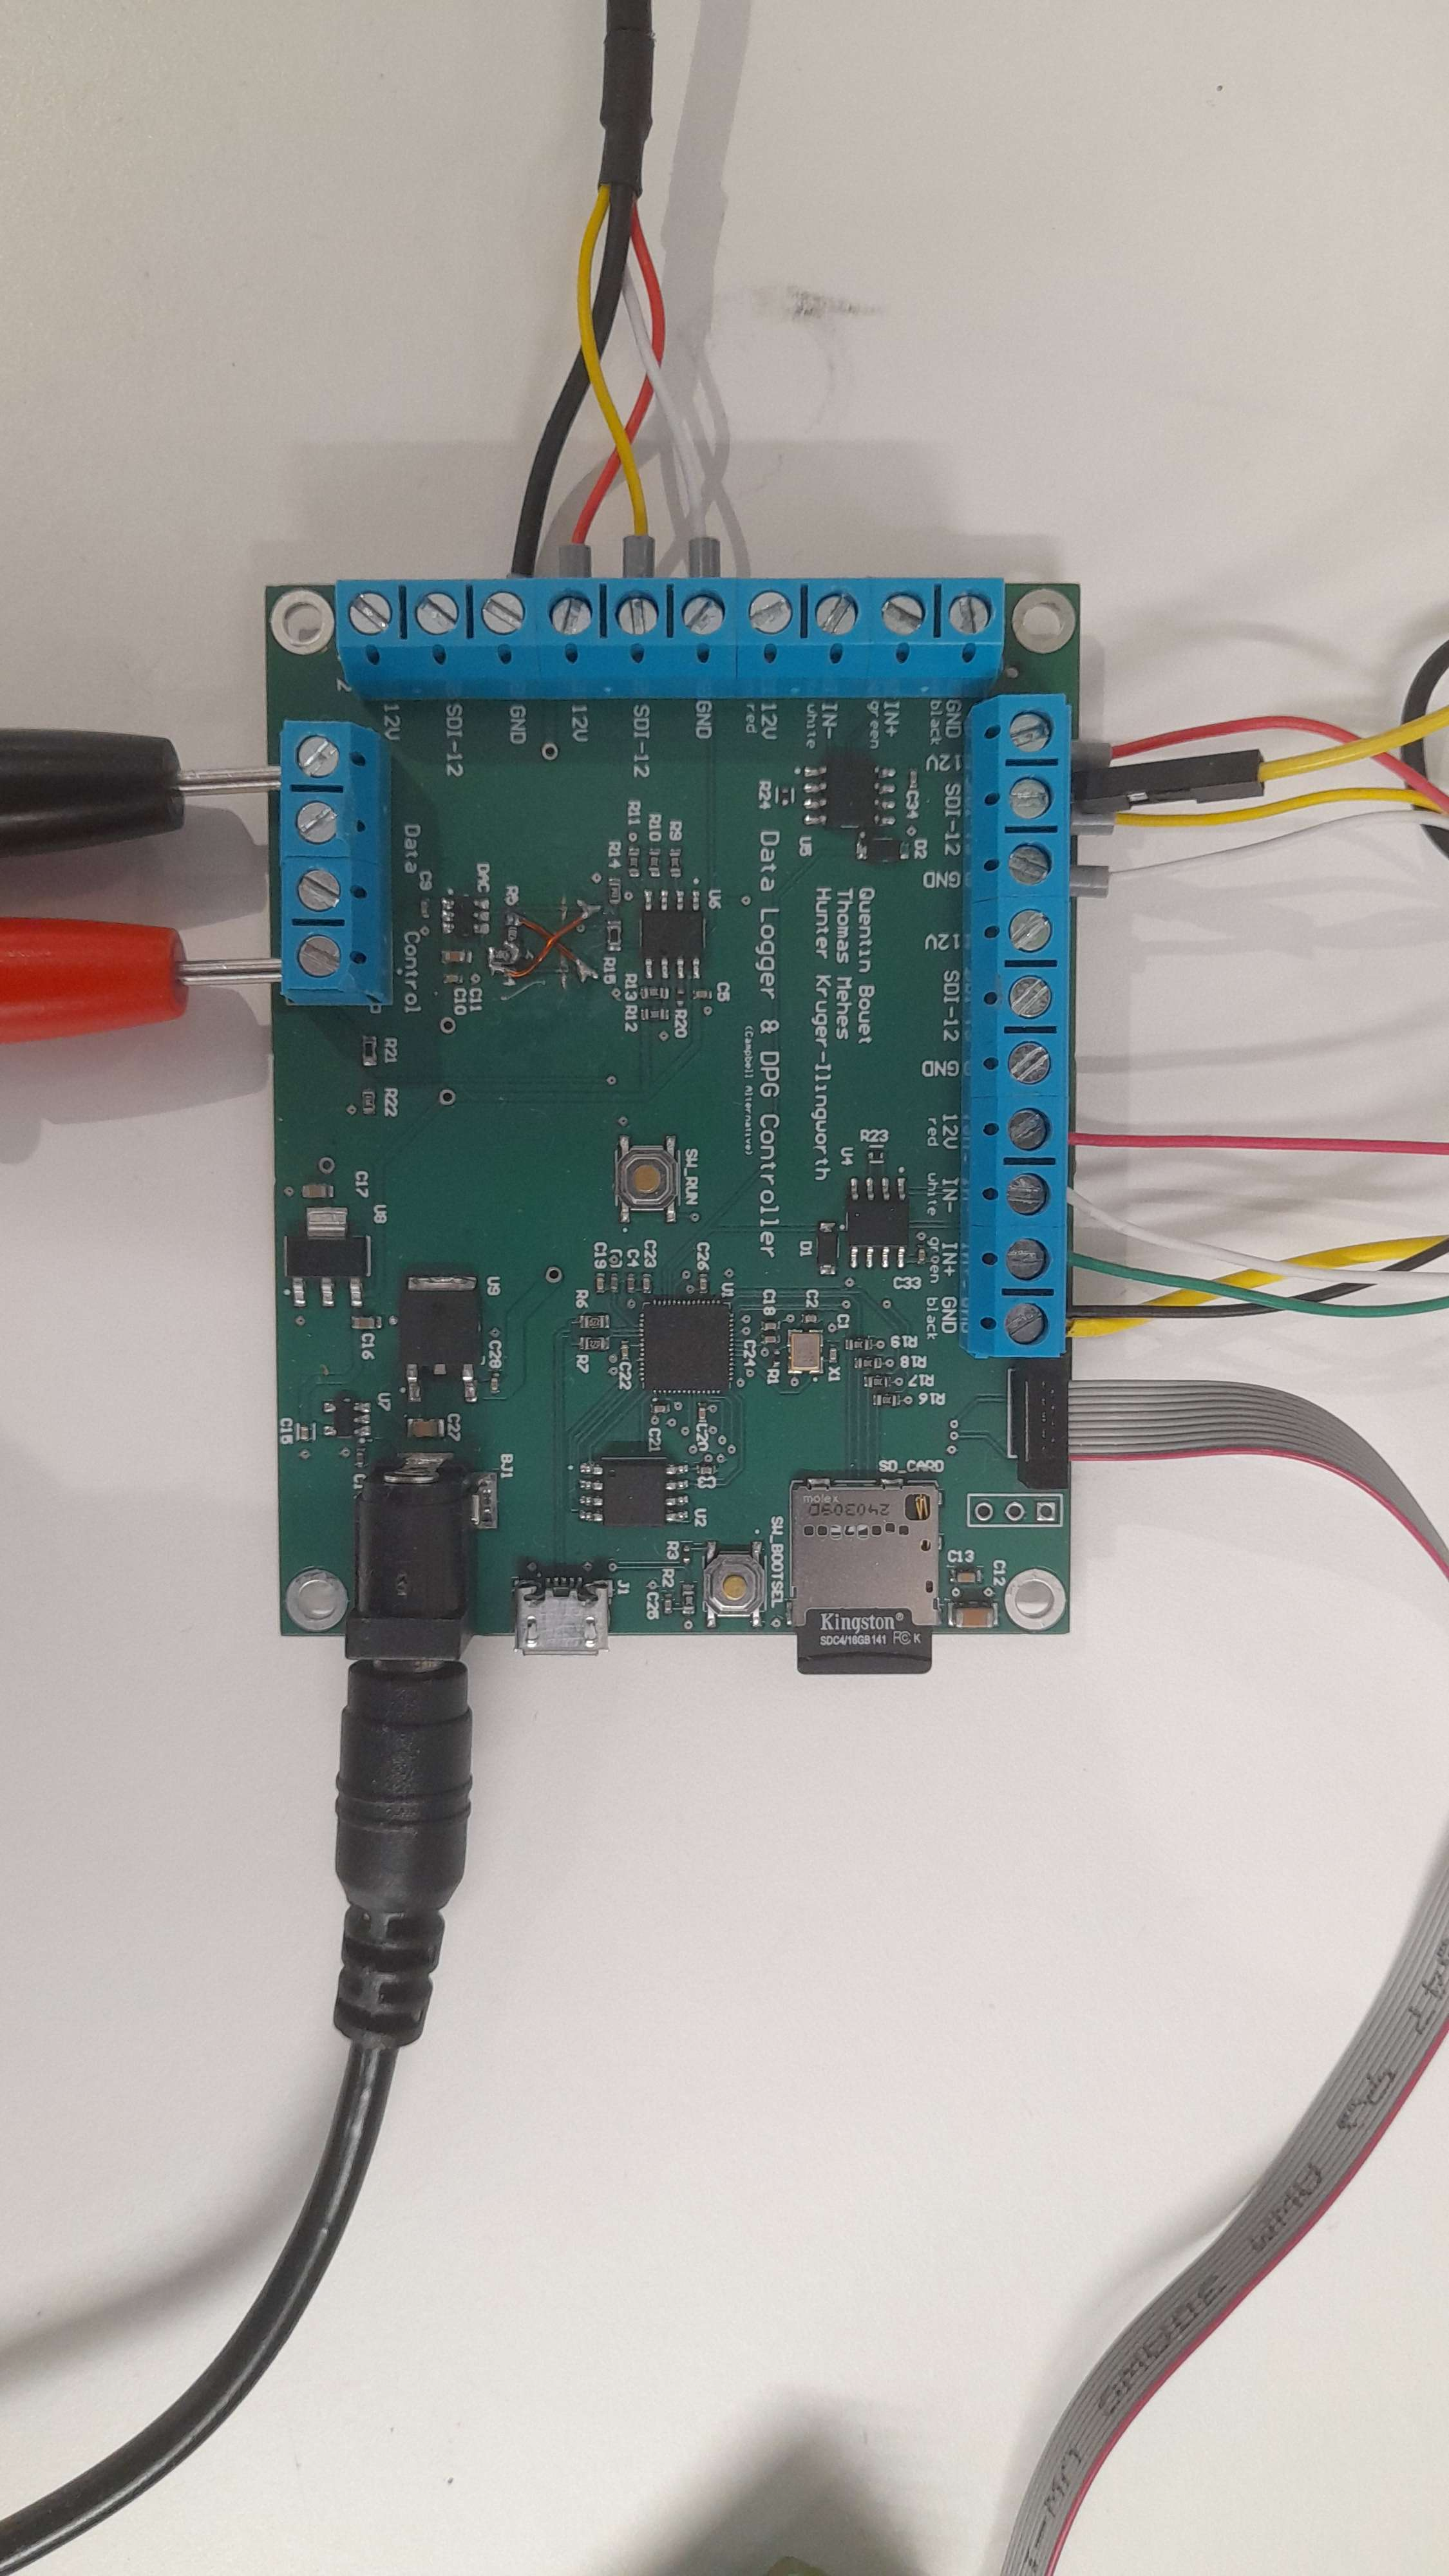
\includegraphics[width=0.4\linewidth]{figures/board_photo.jpg}
    \caption{Photo of Board}
    \label{board_photo}
\end{figure}

\begin{figure}
    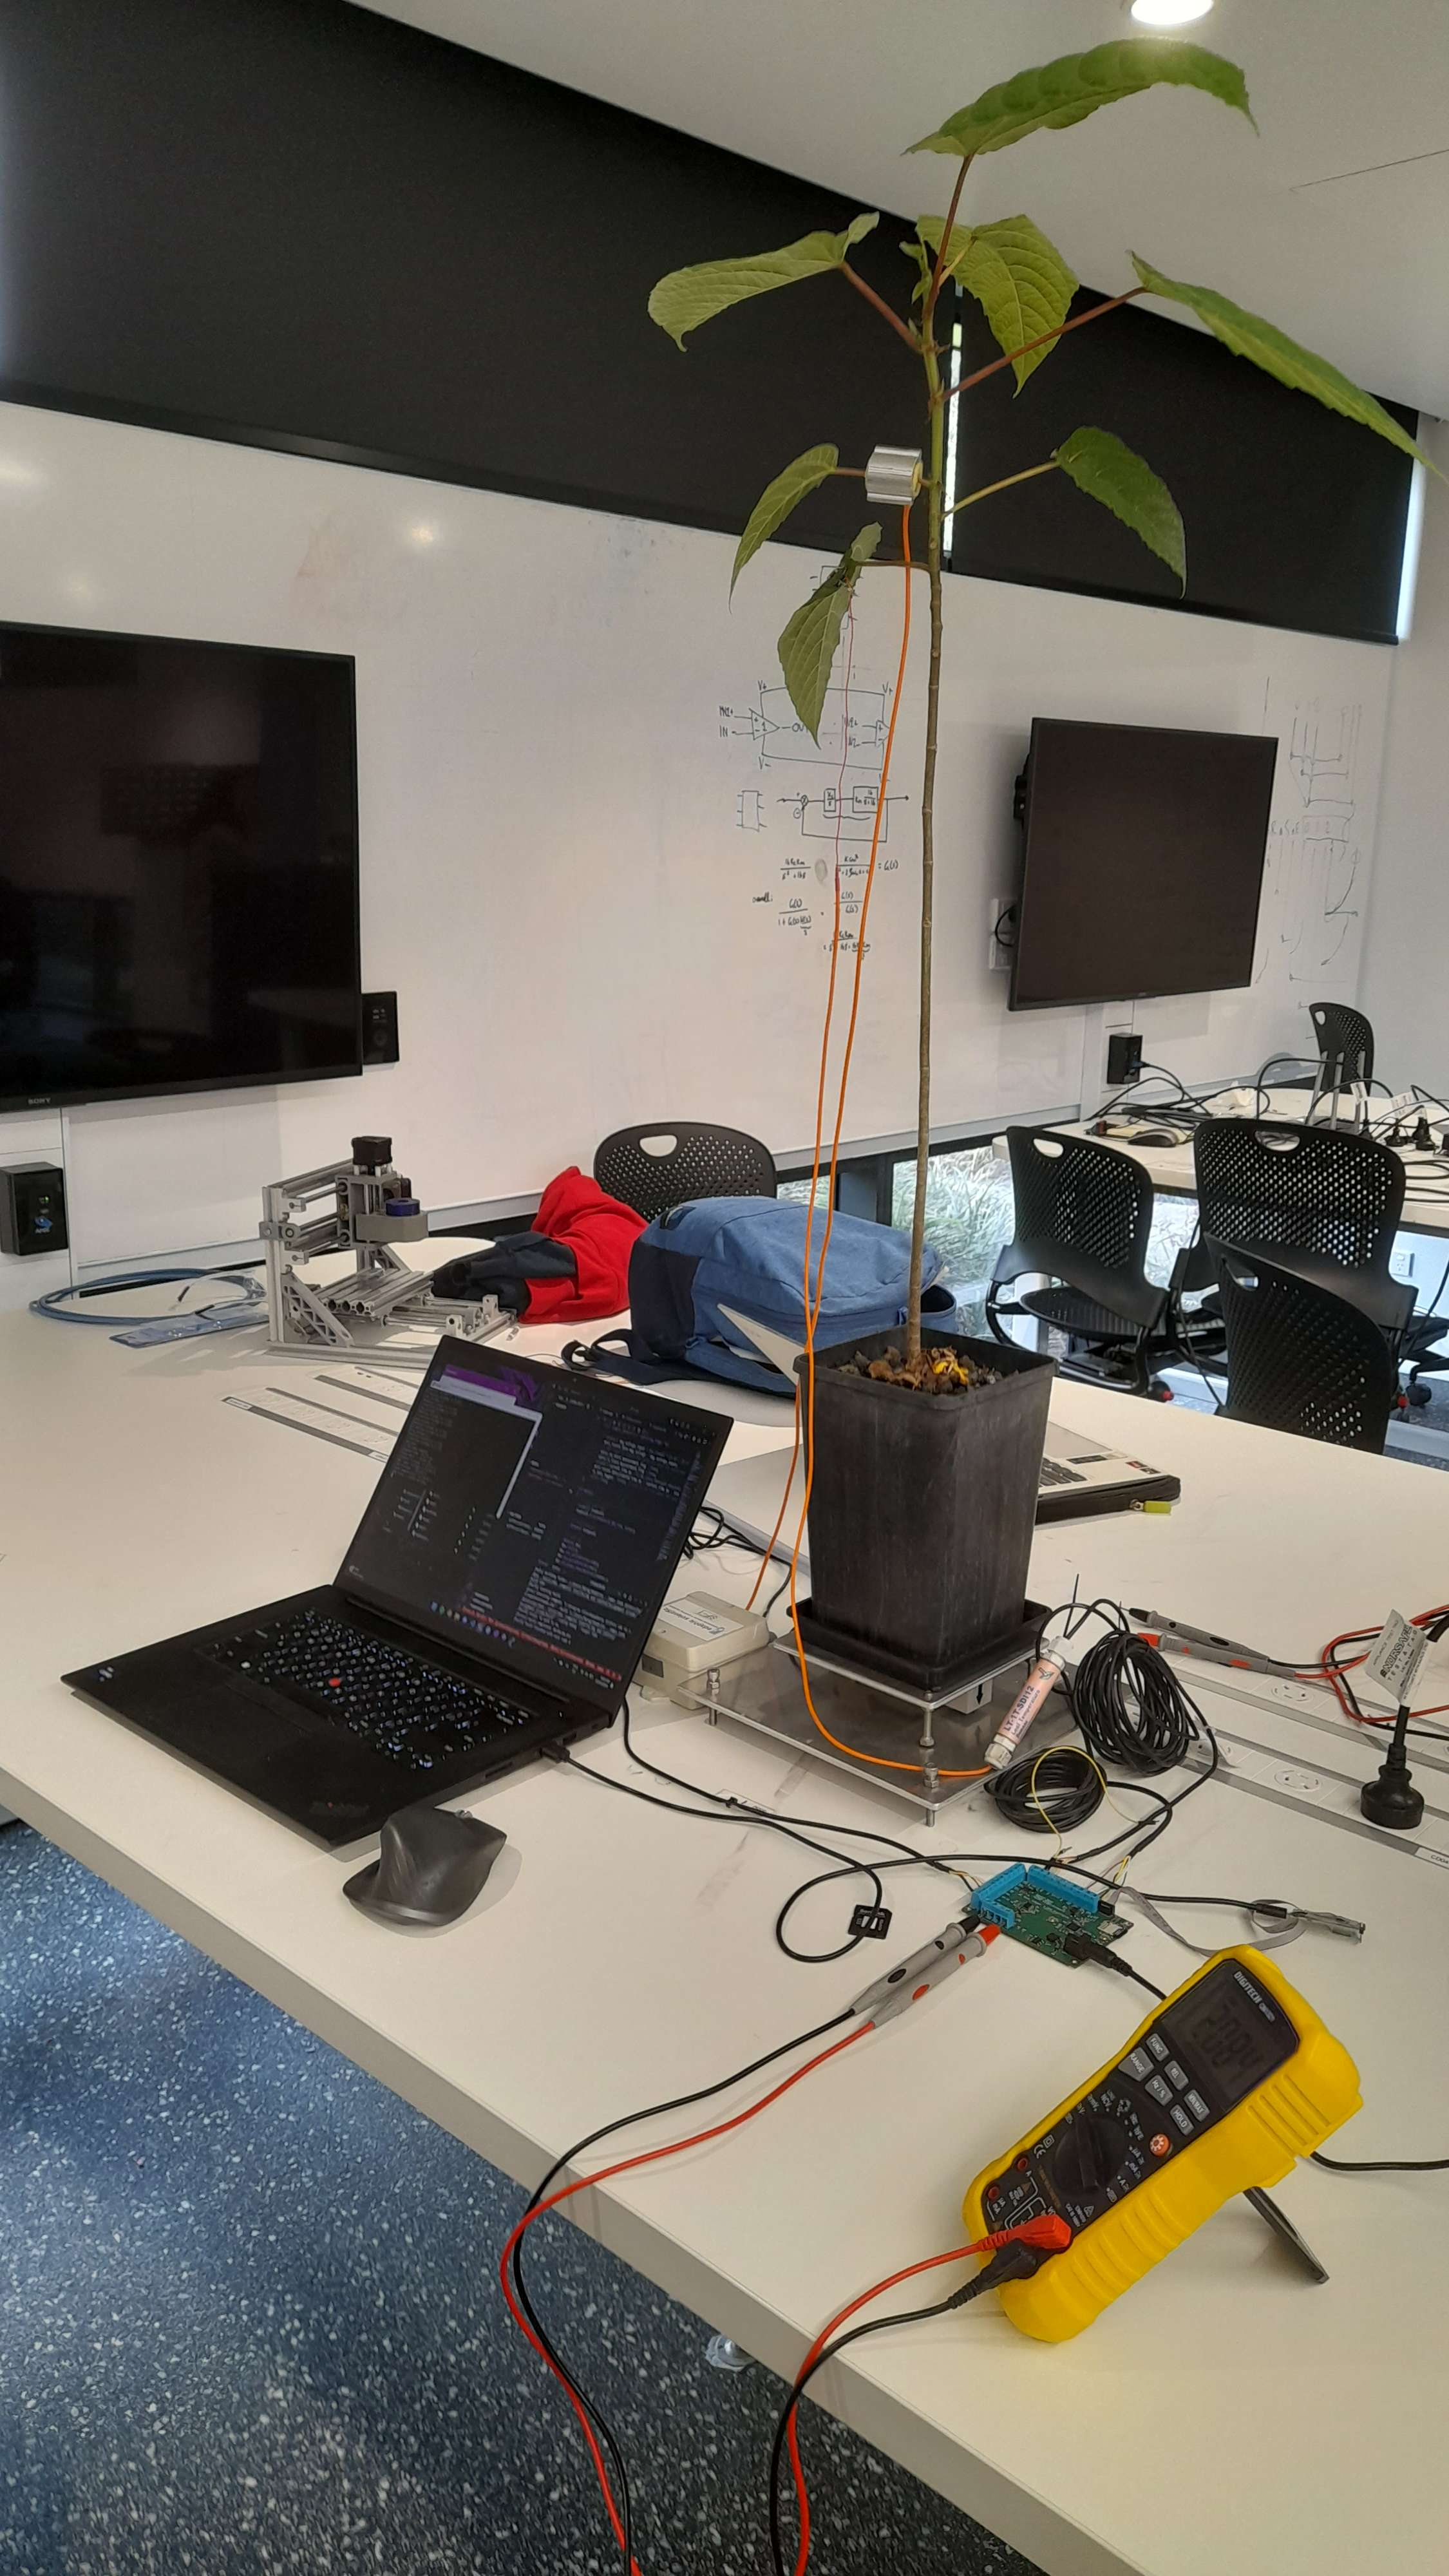
\includegraphics[width=0.4\linewidth]{figures/system_setup_1.jpg}
    \caption{Photo of System Setup}
    \label{system_photo}
\end{figure}


    \subsection{Communication Protocols and OSI Model Layers}

In designing the embedded system, several communication protocols were implemented 
to interface with various sensors and peripherals. Understanding how these protocols 
map onto the OSI model layers, particularly the physical and data link layers, is 
crucial for ensuring reliable and efficient data transmission. This section explains 
the OSI model implementation for each protocol used: SDI-12/UART/RS485, SPI, I2C, 
and analog inputs and outputs.

\subsubsection{SDI-12/UART/RS485 Communication}

\textbf{Physical Layer}

SDI-12 communication is managed using UART1 on the RP2040 microcontroller, with specific 
GPIO pins defined for transmission (TX on GPIO 8), reception (RX on GPIO 9), and data 
line drive enablement (GPIO 15). The SDI-12 protocol operates over a single data line 
with negative logic levels, where a logic '0' is represented by a voltage high, and a 
logic '1' by a voltage low. The RS485 transceiver adapts the UART signals to meet these requirements.

The RS485 transceiver is suitable for this application due to its robust communication capabilities:

\begin{itemize}
    \item Noise Immunity: RS485 uses differential signaling, enhancing noise immunity and allowing 
    reliable communication over long distances, which is essential in environmental monitoring setups.
    \item Line Driving Capability: It can drive long cables with high capacitance, ensuring signal 
    integrity between the microcontroller and sensors.
    \item Inverted Logic Handling: The transceiver accommodates the inverted logic levels required by SDI-12 devices.
\end{itemize}

By using only the non-inverting line of the RS485 transceiver and setting appropriate voltage references, 
the system effectively adapts the standard UART interface to meet the physical layer requirements of the SDI-12 protocol.

\textbf{Data Link Layer}

At the data link layer, the SDI-12 protocol defines the communication between the data recorder 
(master) and the sensors (slaves). It operates at 1200 baud with 7 data bits, even parity, and one 
stop bit. The protocol specifies a set of ASCII commands for initiating measurements, requesting 
data, and managing sensor addresses.

In the current implementation, the system communicates with two SDI-12 sensors whose addresses are 
hardcoded. This approach simplifies the software but limits the system's scalability and flexibility. 
SDI-12 allows for up to ten sensors on a single data line, each with a unique address. A more extensible 
system would implement a discovery process using the SDI-12 "Address Query" command (?!) to identify 
all connected sensors dynamically. This would enable the system to communicate with any number of sensors 
without prior knowledge of their addresses, fully utilizing the hardware's capability for extensibility.

\textbf{Application Layer}

Custom drivers were developed for each sensor, adhering to the SDI-12 
protocol. Specific issues with the byte framing of the SDI-12 protocol were addressed by using the 
\code{uart_set_format()} function to configure the communication format correctly, allowing the RP2040 
to receive the inverted data without additional circuitry. The \code{uart_break()} function was used to 
send the break signal while the \code{uart_read_stuff()} function was used to read the response from 
the sensor. The response was then parsed to get the data. The timing of the SDI-12 protocol is shown 
in \cref{sdi12_timing}.

\begin{figure}
    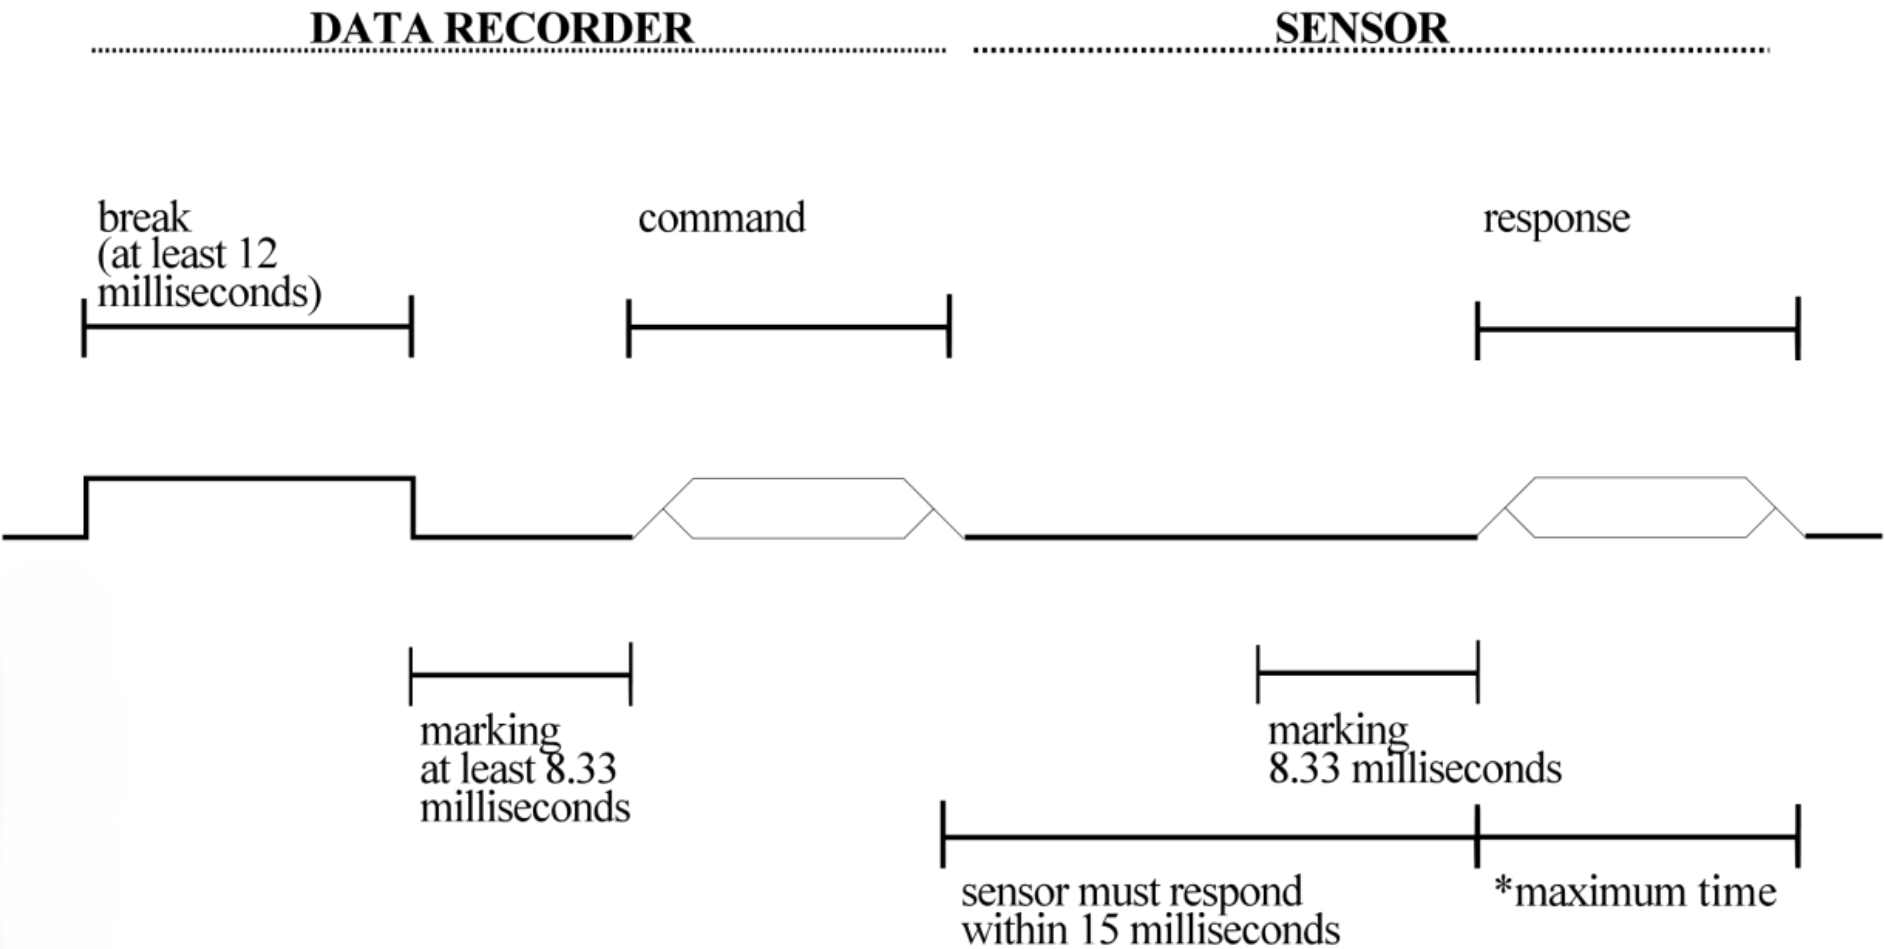
\includegraphics[width=\linewidth]{figures/SDI-12_timing.png}
    \caption{SDI-12 timing from \cite{sdi12_datasheet}}
    \label{sdi12_timing}
\end{figure}

\subsubsection{SPI Communication (SD Card)}

\textbf{Physical Layer}

The SPI protocol is used for communication with the SD card module. SPI is a synchronous serial communication 
interface that operates in full-duplex mode. It uses four signals:
\begin{itemize}
    \item MOSI (Master Out Slave In): Transfers data from the master to the slave.
    \item MISO (Master In Slave Out): Transfers data from the slave to the master.
    \item SCK (Serial Clock): Synchronises data transmission between the master and slave.
    \item SS (Slave Select): Enables the slave device for communication.
\end{itemize}
In this system, the SPI bus operates at a clock speed of 1 MHz, suitable for reliable data transfer 
with the SD card.

\textbf{Data Link Layer}

At the data link layer, the SPI protocol manages the exchange of data bytes between the microcontroller 
and the SD card. It does not define a specific frame format or error-checking mechanism, relying on 
higher-level protocols for these functions. The FatFs file system library is employed to handle file 
operations on the SD card. FatFs provides functions for reading, writing, and managing files, ensuring 
data integrity and proper formatting according to the FAT file system standards.

\textbf{Application Layer}

The FatFs API was integrated to enable read/write operations on the SD card, 
using the SPI protocol. This allowed for structured data logging and easy retrieval of information. 
Functions were implemented to write data in CSV format, facilitating compatibility with data analysis tools.

\subsubsection{I2C Communication (DAC)}

\textbf{Physical Layer}

The I2C protocol is used for communication with the MCP4716 DAC. I2C is a synchronous, multi-master, 
multi-slave, single-ended serial communication bus. It uses two bidirectional open-drain lines:
\begin{itemize}
    \item SDA (Serial Data Line): Transfers data between devices.
    \item SCL (Serial Clock Line): Provides the clock signal for synchronisation.
\end{itemize}
Pull-up resistors are used on both lines to maintain the high logic level when the bus is idle. 
In this system, the I2C bus operates at a standard mode speed of 100 kHz.

\textbf{Data Link Layer}

At the data link layer, the I2C protocol handles addressing and data transfer between the master 
(RP2040 microcontroller) and the slave device (DAC). Each device on the I2C bus has a unique 7-bit address. 
The protocol defines start and stop conditions, acknowledgments, and data byte transfers. The software includes drivers to configure the DAC's settings, such as reference voltage and gain, and to send digital values that the DAC converts into analog voltages. This allows precise control over the dew point generator.

\subsubsection{Analogue Inputs and Outputs}

\textbf{Physical Layer}

Analog inputs and outputs are used to interface with devices like the load cell (MT-603) and the dew point 
generator (LI-610). The load cell produces an analog voltage proportional to the applied weight, which is 
connected to the RP2040's ADC pins. An instrumentation amplifier (e.g., INA826) is used to amplify the small 
signal from the load cell. The dew point generator accepts a 0–5 V analog input for control, which is 
provided by the DAC's output.

\textbf{Data Link Layer}

In the context of analog signals, there is no formal data link layer as in digital communication protocols. 
However, signal conditioning and conversion processes serve similar functions. For analog inputs, the signal 
from the load cell is amplified and filtered before being digitized by the ADC. For analog outputs, the DAC 
converts digital values from the microcontroller into precise analog voltages to control the dew point 
generator's settings.

\textbf{Application Layer}

A software interface for controlling the dew point generator was implemented 
using the I2C protocol to communicate with the DAC. This interface allows precise voltage adjustments to 
the generator, with preliminary tests confirming accurate output predictions based on command inputs. 
The I2C communication was established using standard mode at 100 kHz, which is compatible with the MCP4716 DAC.

The careful selection of communication interfaces and voltage levels, along with robust software 
integration, allowed the system to operate seamlessly and efficiently, providing a reliable solution 
for monitoring and controlling environmental parameters.


    \section{Technical Challenges and Solutions}

\subsection{SDI-12 Sensor Communication Issues}
During the testing of the SDI-12 sensors, initial attempts to communicate using RS485 transceivers failed due to improper framing of byte streams. The strict timing requirements of the SDI-12 protocol made it difficult to achieve reliable communication using standard UART settings. This issue was addressed by applying the \code{uart_set_format()} function, which allowed the RP2040 to handle the SDI-12 protocol's timing more accurately. Additionally, a \code{custom is_timed_out()} function was created to automate character reception without using traditional sleep methods, ensuring precise byte timing and avoiding data loss during transmission.

\subsection{Load Cell Signal Scaling and Stability}
The MT-603 load cell exhibited a significant dead zone and provided inconsistent readings due to mechanical vibrations in the experimental setup. Software-based noise reduction techniques, such as averaging past data points, were implemented to mitigate the effect of oscillations. This software solution was preferred over hardware filtering due to the constraints of the existing apparatus.

\note{Issues with clk and data lines being connected the wrong way around on the RP2040}
    \section{Discussion}

\lipsum[1]

    \section{Recommendations}

Based on the design process and challenges encountered, several recommendations can be made for future engineers who might revise this work:

1. Implement Dynamic Sensor Discovery: To enhance the system's scalability and flexibility, incorporate the SDI-12 "Address Query" command (?!) to dynamically discover all connected sensors. This would eliminate the need for hardcoded sensor addresses and allow the system to support any number of SDI-12 sensors without software modifications.

2. Develop Robust Error Handling: Improve the software to handle communication errors, sensor timeouts, and unexpected responses. Implementing retries, acknowledgments, and exception handling will make the system more reliable in field conditions.

3. Optimize Hardware Design for Extensibility: Ensure that hardware interfaces, such as screw terminals and connectors, are designed to accommodate future expansions. Consider modular designs that allow for easy addition or replacement of components.

4. Thorough PCB Layout Review: Implement a rigorous design review process before finalizing the PCB layout. This includes checking pin assignments, signal integrity, and component placements to prevent issues like swapped pins or incorrect resistor sizing.

5. Enhanced Signal Conditioning: For analog inputs like the load cell, consider implementing hardware filtering and shielding to reduce noise and improve signal stability. This might include adding low-pass filters or using differential signal processing techniques.

6. Documentation and Standardization: Maintain comprehensive documentation of both hardware and software components. Adhering to coding standards and providing clear comments will facilitate future development and maintenance.

7. Power Management: Explore power-saving features and strategies, especially if the system is to be deployed in remote locations where power availability is limited.

By addressing these areas, future iterations of the system can achieve greater robustness, scalability, and ease of use, ultimately enhancing its value for environmental research applications.
    \section{Conclusion}

\note{This section will summarize the project's outcomes, reflecting on the objectives achieved and providing final thoughts.}
    \section{Appendix}




    \bibliographystyle{IEEEtranN} 
    \bibliography{references} 

\end{document}